%-----------------------------------------------------------------------------%
\chapter{\babTiga}
%-----------------------------------------------------------------------------%

This chapter explains the design and analysis of the \code{JSONField}
implementation, as well as \code{JSONField} data validation examples.

%-----------------------------------------------------------------------------%
\section{\code{JSONField}}
%-----------------------------------------------------------------------------%

There are two kinds of \code{JSONField}: the model field and the form field.
The model field is used as an abstraction of the JSON data in the database,
which lets its users manipulate JSON data in the form of Python objects.
The form field is used for accepting JSON data in forms, such as a Django
\code{ModelForm}. Both fields can be validated using Django's built-in
validation feature with custom-made validator functions.

The model field holds JSON data that can be stored to and retrieved from the
database. In Python, the data is represented in Python's built-in formats:
dictionaries, lists, strings, numbers, booleans, and \code{None}. When saving
the model, Django executes an SQL \code{INSERT} or \code{UPDATE} query to the
database. In order to pass the JSON data in the SQL query, the data has to be
serialized into a JSON-encoded string. When retrieving the model instance,
Django executes an SQL \code{SELECT} query to the database. The data is
retrieved as a JSON-encoded string, which needs to be deserialized, or decoded,
into a Python object.

Python has a built-in \code{json} library that can be used to encode/decode
Python objects into/from JSON-encoded strings \cite{python:json}. The encoding
and decoding functionalities are provided through the \code{json.dumps()} and
\code{json.loads()} functions, respectively, as shown in
\autoref{fig:encodecode}. By default, the \code{json.dumps()} function uses the
\code{json.JSONEncoder} class, while the \code{json.loads()} function uses the
\code{json.JSONDecoder} class. These classes support the Python \code{dict},
\code{list}, \code{str}, \code{int}, \code{float}, \code{True}, \code{False},
and \code{None} data types and objects. To support other data types and
objects, customized \code{json.JSONEncoder} and \code{json.JSONDecoder}
subclasses can be used for the functions by supplying the subclass as the
\code{cls} argument.

\begin{figure}
	\centering
    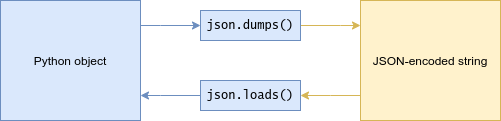
\includegraphics[width=0.66\textwidth]{pics/encodecode.png}
	\caption{The use of the \code{json.dumps()} and \code{json.loads()}
	functions to encode a Python object and decode a JSON-encoded string,
	respectively.}
	\label{fig:encodecode}
\end{figure}

The form field utilizes the \code{json} library for serialization and
deserialization when handling JSON input from the client. If the data being
deserialized is not a valid JSON document, the \code{json.loads()} function
will raise a \code{JSONDecodeError}. This error is used by Django to provide
a basic validation functionality by catching the error and raising a
\code{ValidationError} instead.

\begin{table}
	\centering
	\texttt{
\begin{tabular}{|c|c|c|c|}
\hline
\no{Python}    & \no{JSON} & \no{SQL}            & \no{JSON-encoded string} \\ \hline
'' \no{or} ""  & ""        & ''                  & '""'                     \\ \hline
\{\}           & \{\}      & \no{not applicable} & '\{\}'                   \\ \hline
[]             & []        & \no{not applicable} & '[]'                     \\ \hline
None           & null      & NULL                & 'null'                   \\ \hline
\end{tabular}
}
	\caption{Comparison of empty values and their equivalents in Python, JSON, and SQL.
	The "JSON-encoded string" column shows the Python values after serialization
	with \code{json.dumps()}.}
	\label{table:emptyvalues}
\end{table}

When serializing and deserializing JSON data for the model field, the Python
\code{None} object, the JSON \code{null} value, and the SQL \code{NULL} value
should be taken into consideration. The model field uses JSON-encoded strings
to store JSON values, as there are no SQL equivalents for JSON objects and
arrays. Following the patterns of other values shown in
\autoref{table:emptyvalues}, the \code{None} object should be stored as the
JSON-encoded \code{'null'} string on the database. However, according to the
Python DB-API 2.0 specification (which Django follows), the \code{None} object
is reserved for the SQL \code{NULL} value for both input and output
\cite{db-api2}. Therefore, the model field should skip the serialization and
deserialization for \code{None} (if it's stored as the top-level value) and let
the database driver handle it as SQL \code{NULL}.

In order to store and query the JSON \code{null} value as the top-level value
of \code{JSONField}, the \code{Value} class from the \code{django.db.models}
module can be utilized. A \code{Value()} object wraps a literal SQL value to be
used in an SQL expression \cite{django:value}. This literal SQL value is not
processed by Django. In the case of \code{JSONField}, that means the value is
not passed into the \code{json.dumps()} function. Therefore, the JSON
\code{null} value can be stored as a JSON-encoded SQL string literal (i.e.
\code{Value('null')}), which will be stored as \code{'null'} and not
\code{'"null"'}. However, when the value is retrieved from the database as
\code{'null'}, Django will process the value using \code{json.loads()}, which
will return \code{None}. Meanwhile, when \code{None} is saved back to the
database, it will be saved as SQL \code{NULL}. This behavior may cause
confusion as discussed on the GitHub pull request shown in
\autoref{fig:nulldiscussion}.\footnote{\url{
	https://github.com/django/django/pull/11452\#discussion\_r335375254}}
To avoid this confusion, Django does not recommend working with JSON
\code{null} as the top-level value of JSONField.

\begin{figure}
	\centering
    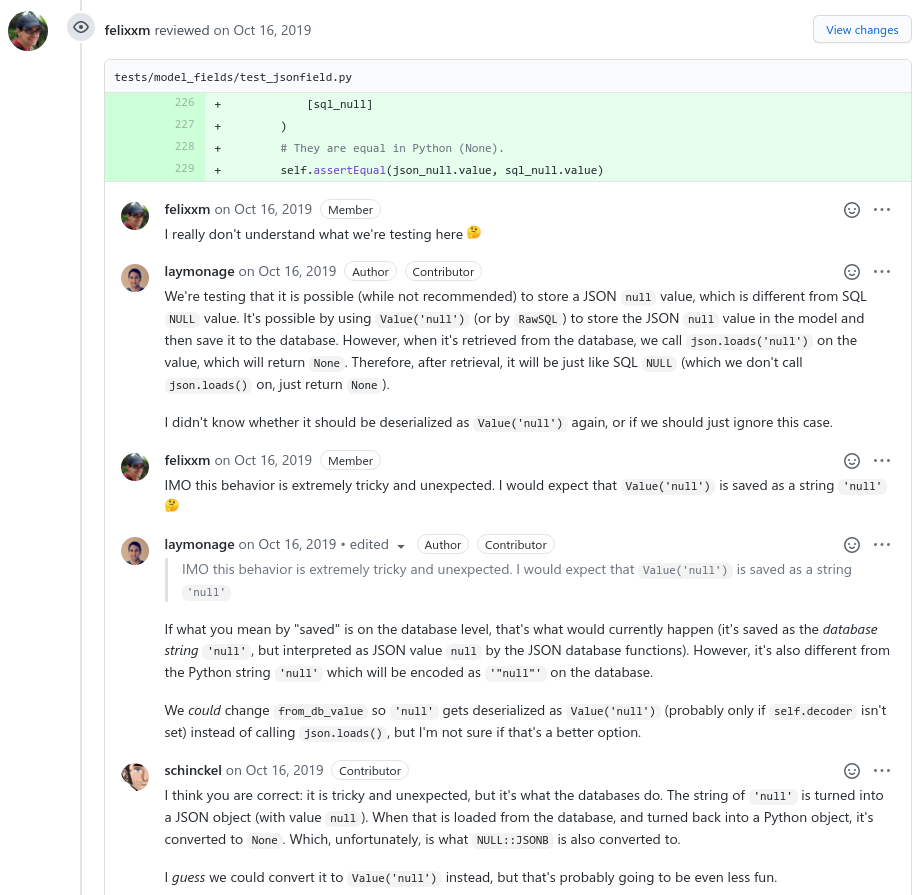
\includegraphics[width=1.0\textwidth]{pics/null_discussion.png}
	\caption{A brief discussion regarding the use of JSON \code{null} as the
	top-level value of a \code{JSONField}.}
	\label{fig:nulldiscussion}
\end{figure}

As with string-based fields such as \code{CharField} and \code{TextField},
Django recommends avoiding the use of SQL \code{NULL} for \code{JSONField}. If
the SQL \code{NULL} is used on a string-based field, it means that there are
two possible values for "no data": \code{NULL} and the empty string
(\code{''}). On \code{JSONField}, it means that there are the empty JSON object
(\code{'\{\}'}), the empty JSON array (\code{'[]'}), the empty JSON string
(\code{'""'}), the JSON \code{null} value (\code{'null'}), and the SQL
\code{NULL}. To avoid redundancy, Django recommends setting \code{null=False}
(to enforce database-level \code{NOT NULL} constraint) and providing a suitable
default for empty values, such as \code{default=dict}.

%-----------------------------------------------------------------------------%
\section{\code{JSONField} Lookups and Transforms}
%-----------------------------------------------------------------------------%

% Containment Lookups

% Key Existence Lookups

% Key, Index, and Path Transforms
